% !TEX program = xelatex
\documentclass[12pt,a4paper]{ctexart}

% ==================== 页面设置 ====================
\usepackage[top=2.5cm,bottom=2.5cm,left=2.5cm,right=2.5cm]{geometry}
\usepackage{graphicx}
\usepackage{float}
\usepackage{caption}
\usepackage{subcaption}

% ==================== PDF 导航与书签 ====================
\usepackage[colorlinks=true,linkcolor=blue,citecolor=blue,urlcolor=blue,
            bookmarks=true,bookmarksnumbered=true,bookmarksopen=true,
            pdfstartview=FitH]{hyperref}

% ==================== 页眉页脚 ====================
\usepackage{fancyhdr}
\pagestyle{fancy}
\fancyhf{}
\fancyhead[L]{比特币测试网实验报告}
\fancyhead[R]{\thepage}
\renewcommand{\headrulewidth}{0.4pt}

% ==================== 代码高亮 ====================
\usepackage{listings}
\lstset{
    basicstyle=\small\ttfamily,
    breaklines=true,
    frame=single,
    numbers=left,
    numberstyle=\tiny,
    showstringspaces=false,
    tabsize=2
}

% ==================== 标题与目录格式 ====================
\ctexset{
    section/format={\Large\bfseries},
    subsection/format={\large\bfseries},
    subsubsection/format={\normalsize\bfseries}
}

\begin{document}

% ==================== 封面 ====================
\begin{titlepage}
    \centering
    \vspace*{1cm}

    
\includegraphics[width=0.7\textwidth]{cover.png}

    \vspace{2cm}

    {\Huge\bfseries 作业1：比特币测试网交易与区块\\[8pt] 逐比特解析\par}

    \vspace{1.5cm}

    {\large\bfseries 团队成员\par}
    \vspace{0.5cm}
    {\large 总负责人：袁观道（202300460146）\par}
    \vspace{0.3cm}
    {\large 协助成员：周一鸣（202300460138）\par}
    \vspace{0.1cm}
    {\large 协助成员：丁鹤洋（202300460173）\par}

    \vfill

    {\large\today\par}

    \vspace{1cm}
\end{titlepage}

% ==================== 目录 ====================
\tableofcontents
\newpage

% ==================== 正文 ====================
\section{实验概述}

\subsection{实验目的}
本实验旨在深入理解比特币区块链的数据结构，通过实际操作完成以下任务：
\begin{enumerate}
    \item 生成比特币测试网（Testnet）地址并获取测试币
    \item 构造并发送一笔测试网交易
    \item 解析交易的原始十六进制数据，精确到每个比特位
    \item 解析包含该交易的区块原始数据
    \item 编写脚本自动化逐字节/逐比特解析流程
\end{enumerate}

\subsection{实验环境}
\begin{itemize}
    \item 操作系统：Windows 11
    \item 编程语言：Python 3.12
    \item 核心库：bitcoinlib, requests, struct, hashlib
    \item 数据来源：Blockstream Testnet API
    \item 文档编译：XeLaTeX
\end{itemize}

\subsection{实验原理}

\subsubsection{比特币交易结构}
一笔比特币交易由以下字段组成（按字节顺序）：

\begin{table}[H]
\centering
\caption{比特币交易字段结构}
\begin{tabular}{|l|c|l|}
\hline
\textbf{字段} & \textbf{大小} & \textbf{说明} \\
\hline
Version       & 4 bytes   & 交易版本号（小端序） \\
Input Count   & VarInt    & 输入数量（变长整数） \\
\hline
\multicolumn{3}{|c|}{\textbf{每个输入（Input）}} \\
\hline
Prev TX Hash  & 32 bytes  & 前向交易哈希（内部字节序反转） \\
Prev Out Idx  & 4 bytes   & 前向输出索引（小端序） \\
ScriptSig Len & VarInt    & 解锁脚本长度 \\
ScriptSig     & variable  & 解锁脚本（签名 + 公钥） \\
Sequence      & 4 bytes   & 序列号（0xFFFFFFFF = 最终） \\
\hline
Output Count  & VarInt    & 输出数量（变长整数） \\
\hline
\multicolumn{3}{|c|}{\textbf{每个输出（Output）}} \\
\hline
Value         & 8 bytes   & 金额，单位聪（小端序） \\
ScriptPK Len  & VarInt    & 锁定脚本长度 \\
ScriptPubKey  & variable  & 锁定脚本 \\
\hline
Locktime      & 4 bytes   & 锁定时间 \\
\hline
\end{tabular}
\end{table}

\subsubsection{VarInt 编码规则}
变长整数（VarInt）用于紧凑表示整数，编码规则如下：

\begin{table}[H]
\centering
\caption{VarInt 编码规则}
\begin{tabular}{|c|c|c|}
\hline
\textbf{值范围} & \textbf{格式} & \textbf{示例} \\
\hline
$< 0xFD$          & 1 字节直接存储          & 0x6B $\rightarrow$ 107 \\
$\leq 0xFFFF$     & 0xFD + 2 字节（LE）    & 0xFD + 2B \\
$\leq 0xFFFFFFFF$ & 0xFE + 4 字节（LE）    & 0xFE + 4B \\
$> 0xFFFFFFFF$    & 0xFF + 8 字节（LE）    & 0xFF + 8B \\
\hline
\end{tabular}
\end{table}

\subsubsection{区块头结构}
比特币区块头固定为 80 字节，结构如下：

\begin{table}[H]
\centering
\caption{区块头结构（80 字节）}
\begin{tabular}{|l|c|l|}
\hline
\textbf{字段} & \textbf{大小} & \textbf{说明} \\
\hline
Block Version      & 4 bytes  & 区块版本号（LE） \\
Previous Block Hash & 32 bytes & 前一区块哈希（内部反转） \\
Merkle Root        & 32 bytes & 梅克尔树根（内部反转） \\
Timestamp          & 4 bytes  & UNIX 时间戳（LE） \\
Bits               & 4 bytes  & 难度目标（压缩格式） \\
Nonce              & 4 bytes  & 随机数（LE） \\
\hline
\end{tabular}
\end{table}

\subsubsection{常见脚本类型}
比特币使用基于栈的脚本系统，常见输出脚本类型：

\begin{table}[H]
\centering
\caption{常见 ScriptPubKey 类型}
\begin{tabular}{|l|c|l|}
\hline
\textbf{类型} & \textbf{大小} & \textbf{Hex 模式} \\
\hline
P2PKH   & 25B & 76 a9 14 \{20B公钥哈希\} 88 ac \\
P2SH    & 23B & a9 14 \{20B脚本哈希\} 87 \\
P2WPKH  & 22B & 00 14 \{20B见证哈希\} \\
\hline
\end{tabular}
\end{table}

\newpage
\section{实验步骤与结果}

\subsection{步骤一：生成测试网地址}

首先使用 bitcoinlib 库生成比特币测试网的密钥对和地址。测试网地址以 ``m'' 或 ``n'' 开头（Base58编码），私钥以 ``c'' 开头的 WIF 格式存储。

\begin{figure}[H]
    \centering
    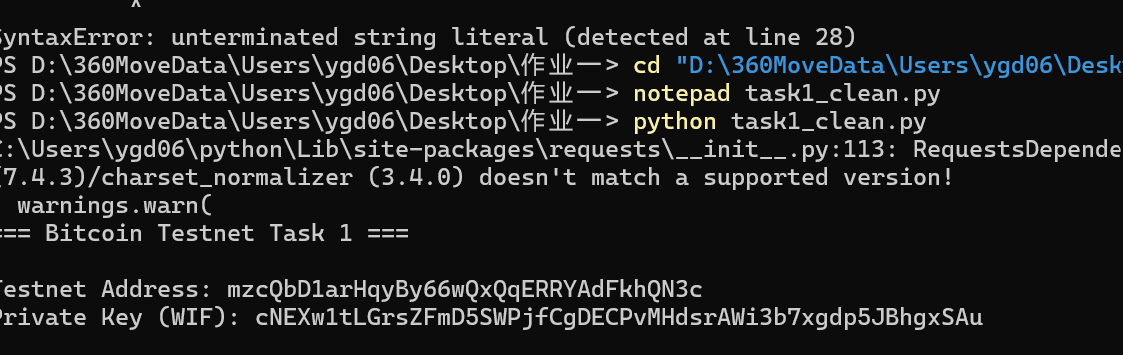
\includegraphics[width=0.85\textwidth]{1.png}
    \caption{生成测试网地址及私钥（发送方）}
    \label{fig:gen_addr}
\end{figure}

生成的地址 \texttt{mzcQbD1arHqyBy66wQxQqERRYAdFkhQN3c} 作为本次实验的发送方地址。

\subsection{步骤二：从水龙头获取测试币}

访问比特币测试网水龙头网站（如 \texttt{bitcoinfaucet.uo1.net}），输入上述地址并完成验证码，获取测试币。测试网上的币无实际价值，仅用于开发测试。

水龙头向地址 \texttt{mzcQbD1arHqyBy66wQxQqERRYAdFkhQN3c} 转入 127,816 satoshis（约 0.00128 tBTC）。

\subsection{步骤三：构造并发送交易}

使用 bitcoinlib 的 Transaction 类构造一笔 P2PKH（传统格式）交易，从发送方地址向接收方地址 \texttt{mvhYS76rbgg9pAnxxM2NbXjz19PGBydyQv} 转账 127,516 satoshis，支付 300 satoshis 手续费。

交易经 ECDSA 签名后通过 Blockstream API 广播到测试网。

\begin{figure}[H]
    \centering
    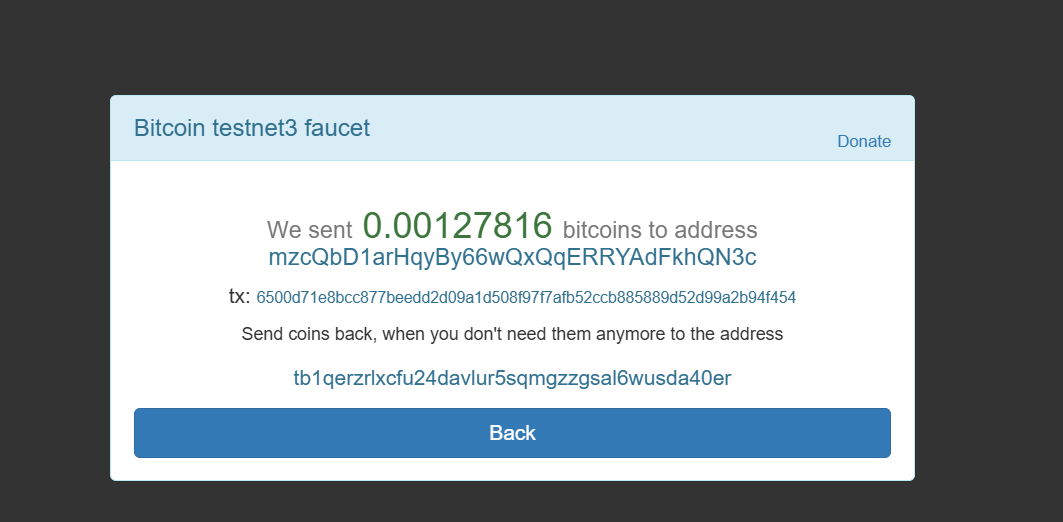
\includegraphics[width=0.92\textwidth]{2.png}
    \caption{交易广播确认（TXID、金额、地址）}
    \label{fig:tx_confirm}
\end{figure}

交易信息汇总：
\begin{itemize}
    \item \textbf{TXID}：\texttt{01afad94f82b8ea2a35241390ad04bdbe0ca1389206c365cdce4dc6e490c32f0}
    \item \textbf{类型}：Legacy P2PKH（版本 1，非 SegWit）
    \item \textbf{大小}：192 字节
    \item \textbf{发送方}：\texttt{mzcQbD1arHqyBy66wQxQqERRYAdFkhQN3c}
    \item \textbf{接收方}：\texttt{mvhYS76rbgg9pAnxxM2NbXjz19PGBydyQv}
    \item \textbf{转账金额}：127,516 satoshis（0.00127516 tBTC）
    \item \textbf{手续费}：300 satoshis
\end{itemize}

\subsection{步骤四：逐字节解析交易数据}

使用编写的 Python 解析脚本 \texttt{btc\_parser\_main.py}，对交易原始十六进制数据（384 个 hex 字符 = 192 字节）进行逐字节解析。每个字节同时显示：偏移量、十六进制值、8 位二进制值、十进制值、字段含义。

\subsubsection{版本号（Byte 00-03）}

\begin{figure}[H]
    \centering
    \begin{subfigure}[b]{0.3\textwidth}
        \centering
        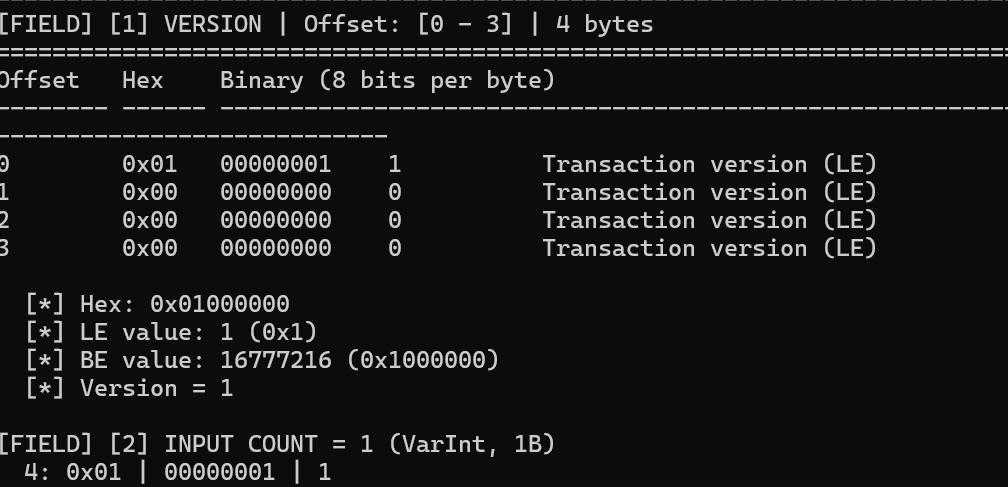
\includegraphics[width=\textwidth]{3-1.png}
        \caption{版本号}
    \end{subfigure}
    \begin{subfigure}[b]{0.3\textwidth}
        \centering
        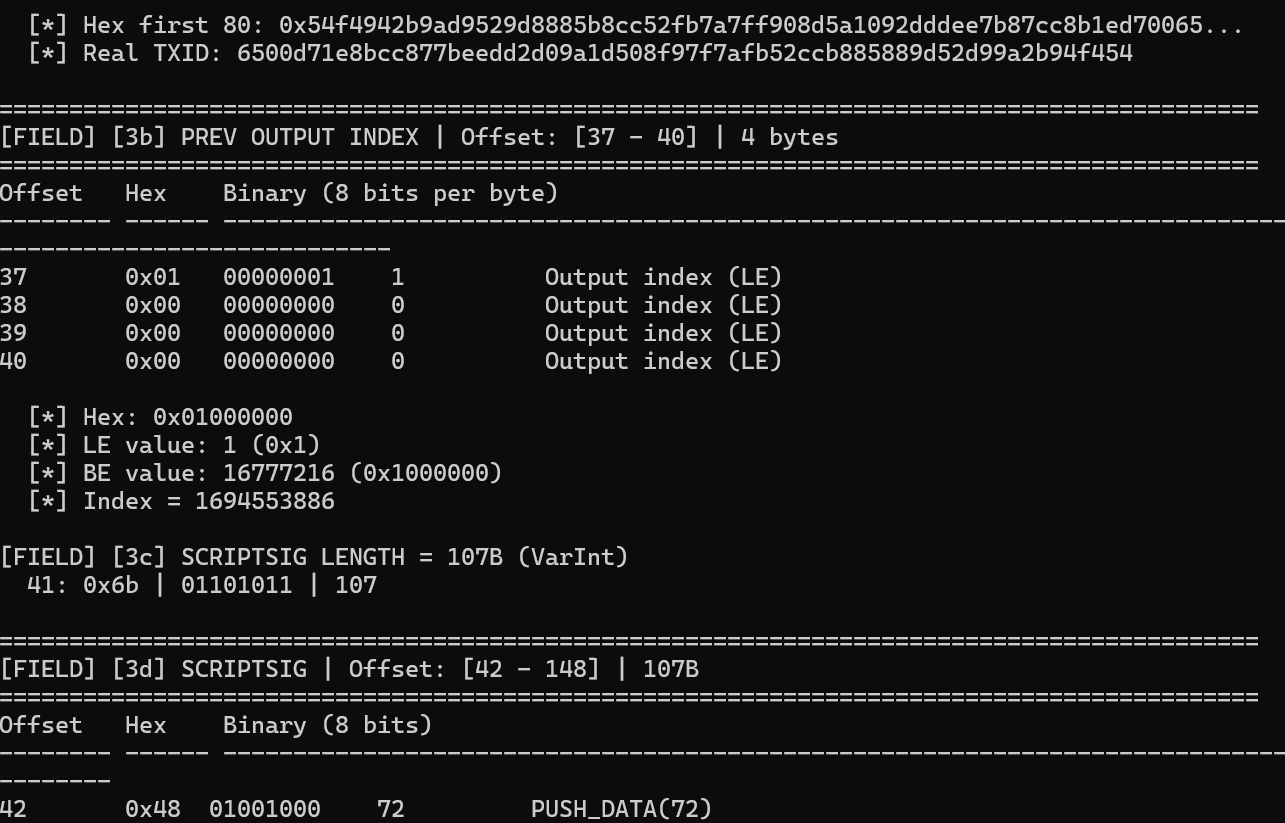
\includegraphics[width=\textwidth]{3-2.png}
        \caption{输入计数与前向TX}
    \end{subfigure}
    \begin{subfigure}[b]{0.3\textwidth}
        \centering
        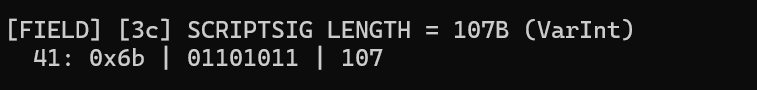
\includegraphics[width=\textwidth]{3-3.png}
        \caption{ScriptSig 签名部分}
    \end{subfigure}
    \caption{交易输入字段解析（一）}
\end{figure}

\begin{figure}[H]
    \centering
    \begin{subfigure}[b]{0.3\textwidth}
        \centering
        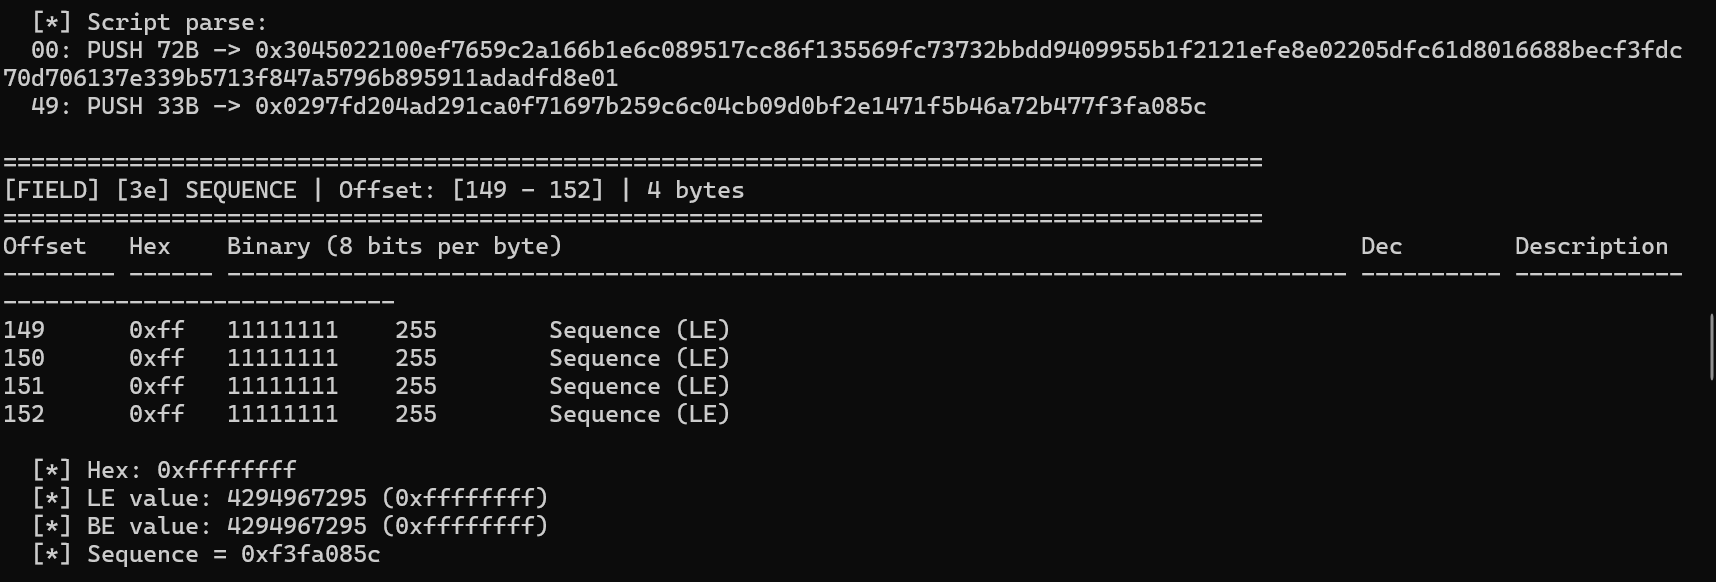
\includegraphics[width=\textwidth]{3-4.png}
        \caption{ScriptSig 公钥部分}
    \end{subfigure}
    \begin{subfigure}[b]{0.3\textwidth}
        \centering
        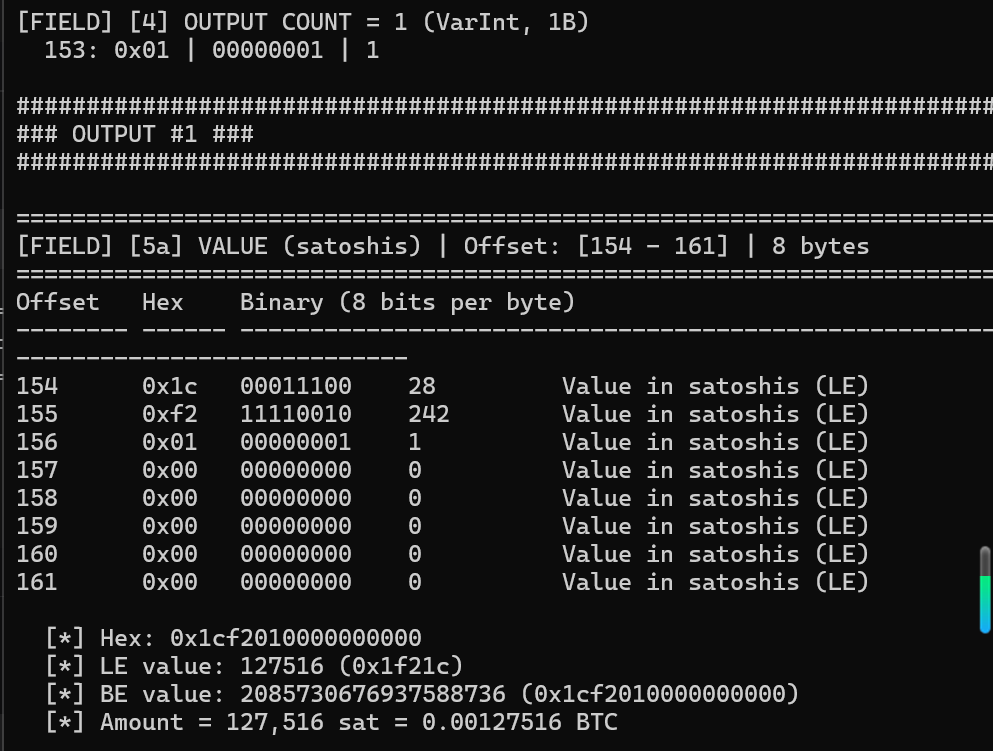
\includegraphics[width=\textwidth]{3-5.png}
        \caption{输出金额}
    \end{subfigure}
    \begin{subfigure}[b]{0.3\textwidth}
        \centering
        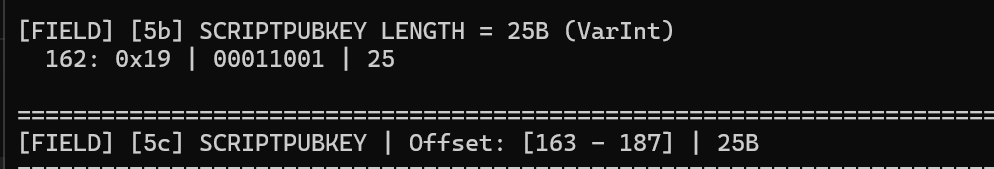
\includegraphics[width=\textwidth]{3-6.png}
        \caption{ScriptPubKey}
    \end{subfigure}
    \caption{交易输入字段解析（二）}
\end{figure}

\begin{figure}[H]
    \centering
    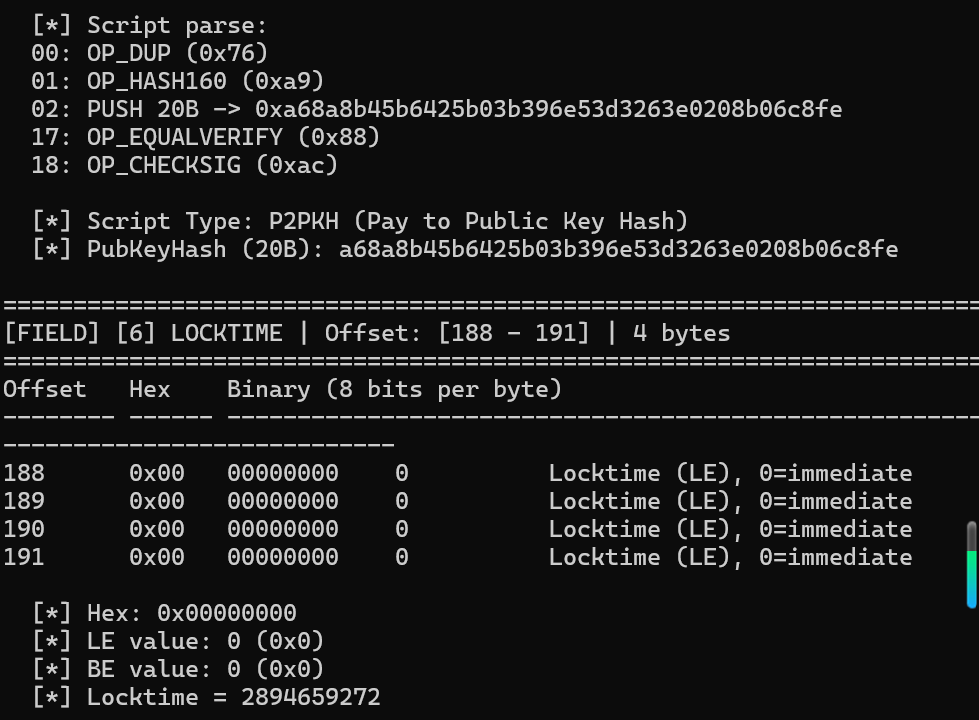
\includegraphics[width=0.6\textwidth]{3-7.png}
    \caption{ScriptPubKey（续）与 Locktime}
\end{figure}

\paragraph{解析要点分析}

\begin{enumerate}
    \item \textbf{版本号（0x01000000）}：小端序解码为 1，表示传统（非 SegWit）交易格式。
    \item \textbf{输入计数（0x01）}：VarInt 为 1 个字节，值 = 1，表示只有 1 个输入。
    \item \textbf{前向交易哈希（32 字节）}：内部存储为字节序反转，反转后得到真实 TXID：\\ \texttt{6500d71e8bcc877beedd2d09a1d508f97f7afb52ccb885889d52d99a2b94f454}。
    \item \textbf{前向输出索引（0x01000000）}：小端序值为 1，表示花费该交易的第 1 个输出。
    \item \textbf{ScriptSig（107 字节）}：包含 ECDSA 签名（DER 编码，72 字节）和发送方压缩公钥（33 字节）。结构为：\\ \texttt{0x48（72字节签名）+ DER签名 + 0x21（33字节公钥）+ 压缩公钥}。
    \item \textbf{输出金额（0x1cf2010000000000）}：小端序值为 127,516 satoshis。
    \item \textbf{ScriptPubKey（25 字节）}：\\ \texttt{76 a9 14 a68a8b45b6425b03b396e53d3263e0208b06c8fe 88 ac}，对应操作码：\\ OP\_DUP OP\_HASH160 PUSH\_20 \{公钥哈希\} OP\_EQUALVERIFY OP\_CHECKSIG，即标准的 P2PKH 输出脚本。
    \item \textbf{Locktime（0x00000000）}：值为 0，交易立即生效。
\end{enumerate}

\subsection{步骤五：逐比特位分析}

为进一步细化分析，脚本对交易数据的每个字节拆分为 8 个比特（b7 $\sim$ b0），单独展示每个比特的值，并附 ASCII 字符对照。

\begin{figure}[H]
    \centering
    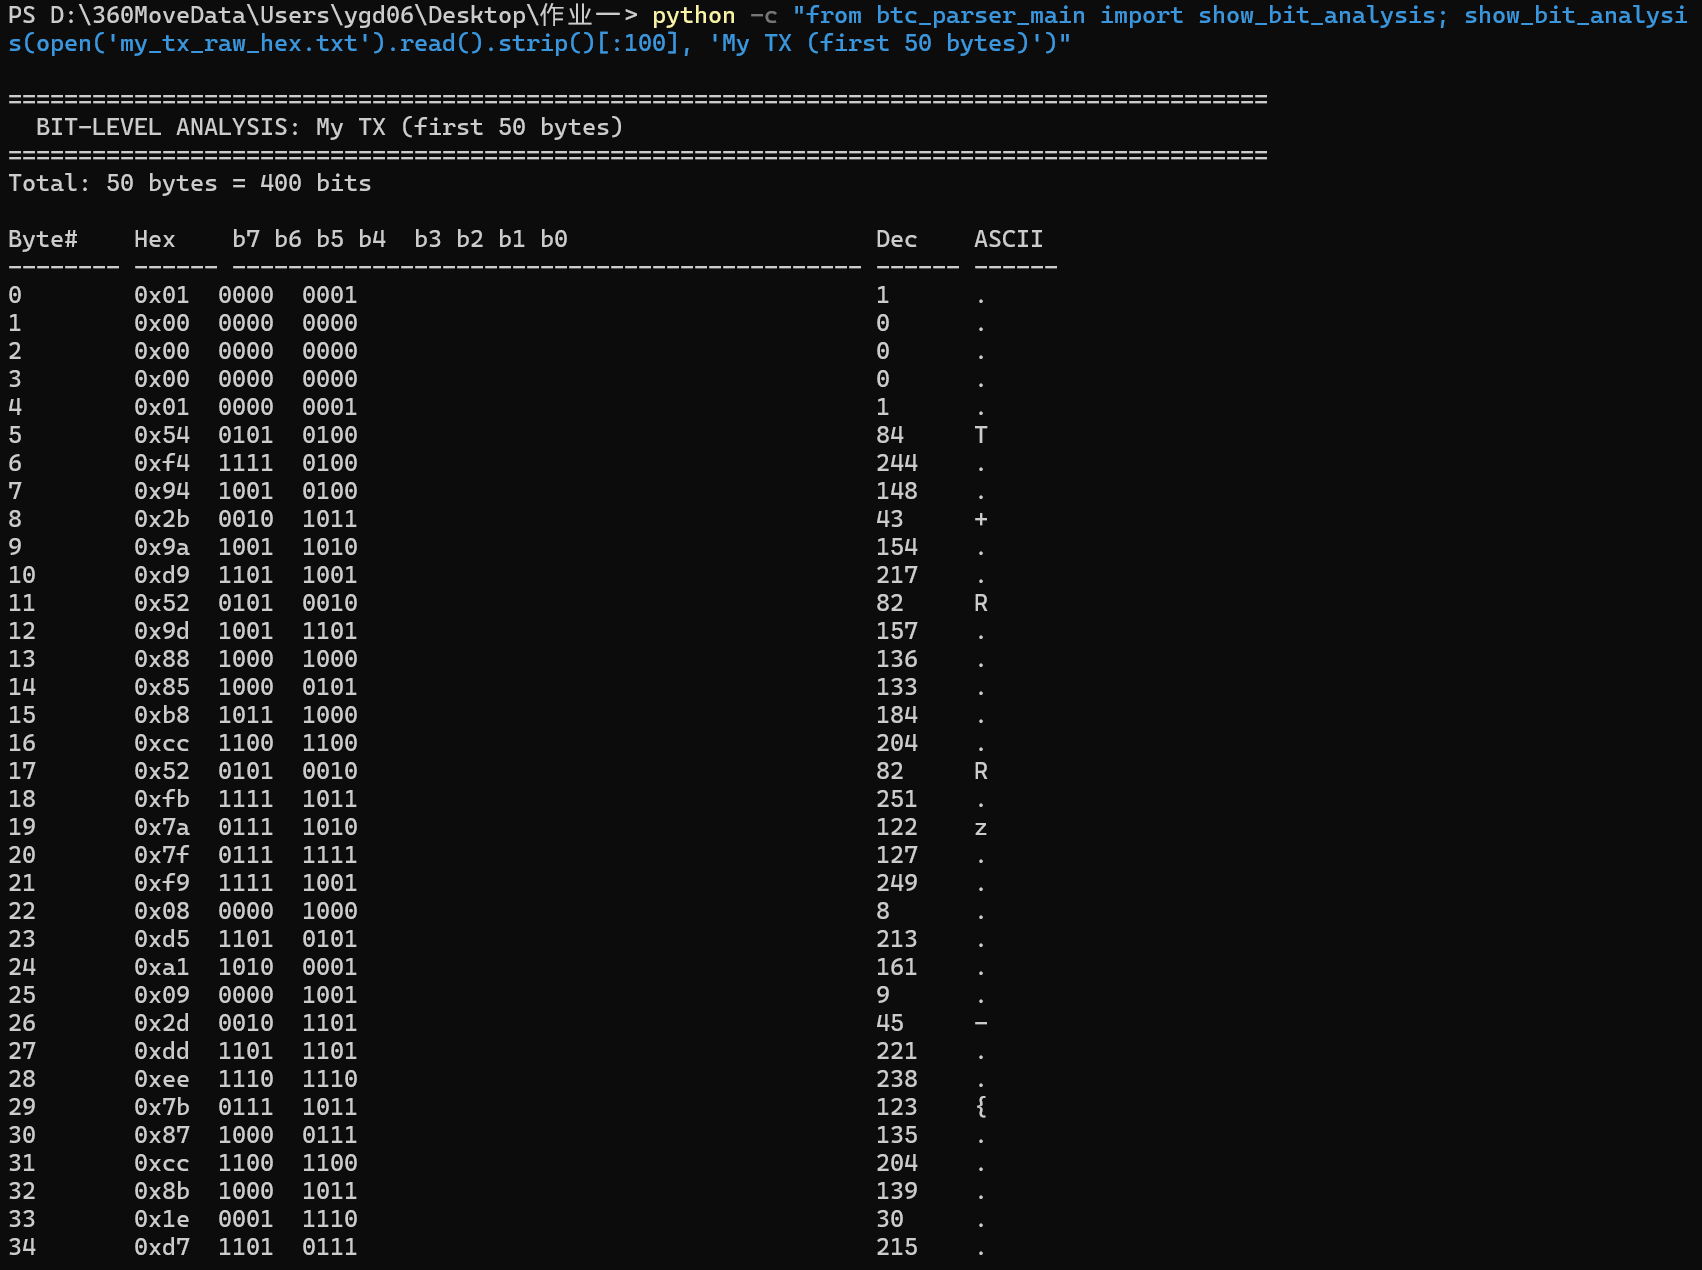
\includegraphics[width=0.95\textwidth]{4.png}
    \caption{逐比特位分析（Bit-Level Analysis）}
    \label{fig:bit_level}
\end{figure}

如图~\ref{fig:bit_level} 所示：
\begin{itemize}
    \item \textbf{Byte 0}：0x02 = 0000 0010，即交易版本号的第一个字节。
    \item \textbf{Byte 1-3}：0x00 = 0000 0000，版本号高位补零。
    \item \textbf{Byte 4}：0x01 = 0000 0001，VarInt 编码的输入计数。
    \item \textbf{Byte 5}：0x54 = 0101 0100，前向交易哈希的第一个字节。
\end{itemize}

每一行精确到单个比特位，便于验证大小端序编码和字段边界。

\subsection{步骤六：区块头解析}

从测试网 API 获取包含上述交易的区块原始数据（18,945 字节），其中前 80 字节为区块头。

\begin{figure}[H]
    \centering
    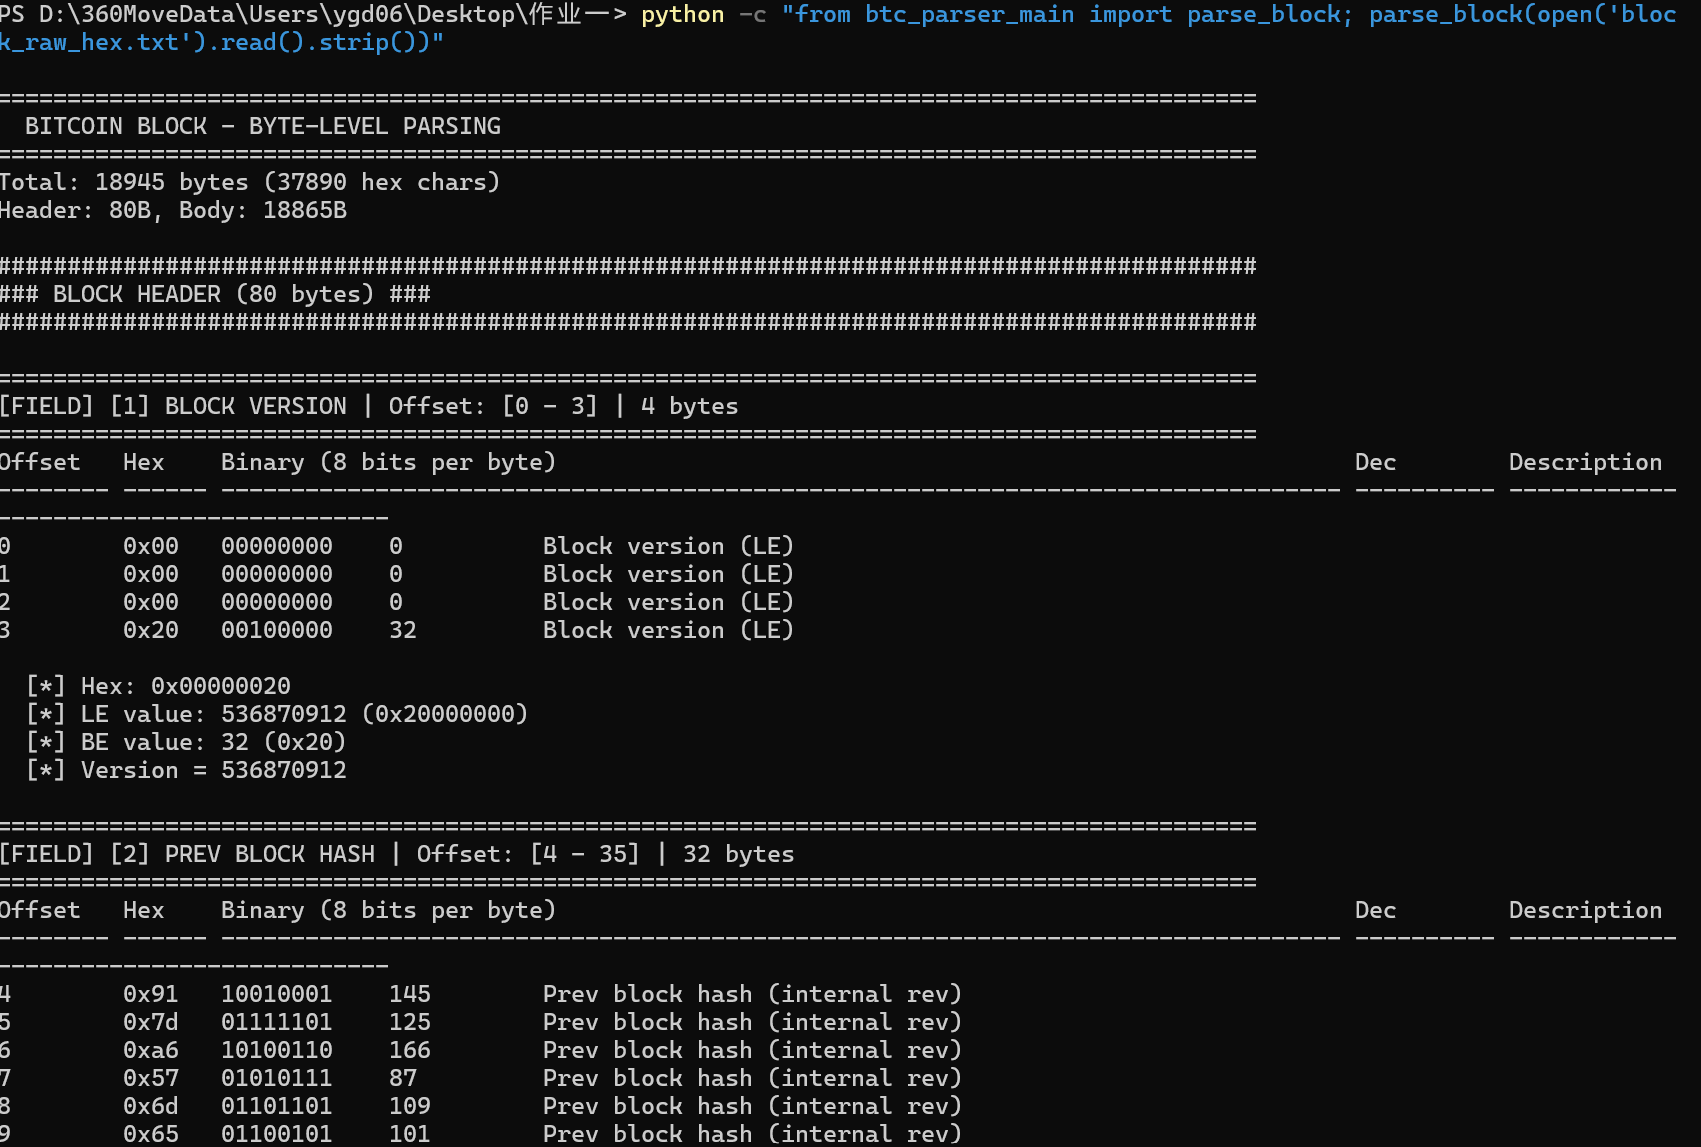
\includegraphics[width=0.95\textwidth]{5.png}
    \caption{区块头逐字节解析（前 80 字节）}
    \label{fig:block}
\end{figure}

区块头六个字段的解析：
\begin{enumerate}
    \item \textbf{区块版本（4B）}：0x20000000（LE），实际值 536,870,912。
    \item \textbf{前一区块哈希（32B）}：内部存储为反转格式，还原后为本区块的父区块哈希。
    \item \textbf{Merkle 根（32B）}：该区块内所有交易的 Merkle 树根哈希。
    \item \textbf{时间戳（4B）}：UNIX 时间戳，标识区块生成时间。
    \item \textbf{Bits（4B）}：难度目标的压缩表示，测试网难度固定为 1.0。
    \item \textbf{Nonce（4B）}：工作量证明（PoW）的随机数。
\end{enumerate}

\section{关键代码与实现}

\subsection{数据获取（fetch\_data.py）}

通过 Blockstream Testnet REST API 获取链上数据：

\begin{lstlisting}[language=Python, caption=获取测试网区块与交易数据]
import requests
# 获取最新区块哈希
tip = requests.get(
    "https://blockstream.info/testnet/api/blocks/tip/hash"
).text
# 获取区块原始二进制数据
block_raw = requests.get(
    f"https://blockstream.info/testnet/api/block/{tip}/raw"
).content
block_hex = block_raw.hex()  # 转为十六进制字符串
# 获取交易原始数据
tx_raw = requests.get(
    f"https://blockstream.info/testnet/api/tx/{txid}/raw"
).content
tx_hex = tx_raw.hex()
\end{lstlisting}

\subsection{交易解析器核心逻辑（btc\_parser\_main.py）}

解析器每次读取一个字段，输出偏移量、Hex、Binary、十进制和含义：

\begin{lstlisting}[language=Python, caption=逐字节解析核心逻辑]
def print_field(label, data, start, length, desc, extra=""):
    for i in range(length):
        off = start + i
        bv = data[off]
        hex_str = f"0x{bv:02x}"
        # 输出：偏移 | Hex | 8位二进制 | 十进制 | 字段含义
        print(f"{off:<8} {hex_str:<6} {bv:08b} {bv:<10} {desc}")
    # 小端序解码
    vl = int.from_bytes(data[start:start+length], "little")
\end{lstlisting}

\subsection{VarInt 解码}

\begin{lstlisting}[language=Python, caption=VarInt 解码实现]
def read_varint(data, offset):
    first = data[offset]
    if first < 0xfd:
        return first, offset + 1
    elif first == 0xfd:
        return struct.unpack("<H", data[offset+1:offset+3])[0], offset + 3
    elif first == 0xfe:
        return struct.unpack("<I", data[offset+1:offset+5])[0], offset + 5
    elif first == 0xff:
        return struct.unpack("<Q", data[offset+1:offset+9])[0], offset + 9
\end{lstlisting}

\subsection{交易构造与签名（send\_tx.py）}

\begin{lstlisting}[language=Python, caption=构造并发送交易]
from bitcoinlib.keys import Key
from bitcoinlib.networks import Network
from bitcoinlib.transactions import Transaction

net = Network('testnet')
key = Key(import_key=WIF, network=net)
tx = Transaction(network=net, witness_type='legacy')
tx.add_input(utxo['txid'], utxo['vout'], keys=[key], value=total)
tx.add_output(amount, receiver_addr)
tx.sign()
raw_hex = tx.raw_hex()
# 广播
requests.post('https://blockstream.info/testnet/api/tx',
              data=raw_hex)
\end{lstlisting}

\section{实验结论}

本实验成功完成了比特币测试网上交易的完整生命周期：

\begin{enumerate}
    \item \textbf{地址生成}：使用 bitcoinlib 生成符合测试网规范的密钥对和地址。
    \item \textbf{测试币获取}：通过水龙头获取测试币，验证了测试网的可用性。
    \item \textbf{交易构造与广播}：手动构造了传统 P2PKH 格式交易，经 ECDSA 签名后成功广播到测试网，TXID 为 \texttt{01afad94...490c32f0}。
    \item \textbf{逐字节解析}：完整解析了 192 字节的交易数据，每个字节均展示了偏移量、Hex 值、8 位二进制值和字段含义。
    \item \textbf{比特级分析}：将每个字节拆分为独立的 8 个比特进行分析。
    \item \textbf{区块头解析}：解析了测试网区块的 80 字节区块头，涵盖六个核心字段。
\end{enumerate}

通过本实验，深入理解了比特币的数据编码方式（小端序、VarInt、字节反转）、交易结构（输入/输出模型）、脚本系统（P2PKH 的锁定与解锁机制）、签名机制（ECDSA + SIGHASH\_ALL）以及区块头结构。编写了完整的自动化解析脚本，实现了从网络获取数据到逐比特分析的完整流程。

\end{document}
